%%%%%%%%%%%%%%%%%%%%%%%%%%%%%%%%%%%%%%%%%
% University Assignment Title Page 
% LaTeX Template
% Version 1.0 (27/12/12)
%
% This template has been downloaded from:
% http://www.LaTeXTemplates.com
%
% Original author:
% WikiBooks (http://en.wikibooks.org/wiki/LaTeX/Title_Creation)
%
% License:
% CC BY-NC-SA 3.0 (http://creativecommons.org/licenses/by-nc-sa/3.0/)
% 
% Instructions for using this template:
% This title page is capable of being compiled as is. This is not useful for 
% including it in another document. To do this, you have two options: 
%
% 1) Copy/paste everything between \begin{document} and \end{document} 
% starting at \begin{titlepage} and paste this into another LaTeX file where you 
% want your title page.
% OR
% 2) Remove everything outside the \begin{titlepage} and \end{titlepage} and 
% move this file to the same directory as the LaTeX file you wish to add it to. 
% Then add \input{./title_page_1.tex} to your LaTeX file where you want your
% title page.
%
%%%%%%%%%%%%%%%%%%%%%%%%%%%%%%%%%%%%%%%%%
%\title{Title page with logo}
%----------------------------------------------------------------------------------------
%	PACKAGES AND OTHER DOCUMENT CONFIGURATIONS
%----------------------------------------------------------------------------------------

\documentclass[12pt]{article}
\usepackage[english]{babel}
\usepackage[utf8x]{inputenc}
\usepackage{amsmath}
\usepackage{graphicx}
\usepackage{url}
\usepackage{textcomp}

\usepackage[colorinlistoftodos]{todonotes}

\begin{document}

\begin{titlepage}

\newcommand{\HRule}{\rule{\linewidth}{0.5mm}} % Defines a new command for the horizontal lines, change thickness here

\center % Center everything on the page
 
%----------------------------------------------------------------------------------------
%	HEADING SECTIONS
%----------------------------------------------------------------------------------------

\textsc{\LARGE University of Texas at Austin}\\[1.5cm] % Name of your university/college
%\textsc{\Large Porting Fast Paxos}\\[0.5cm] % Major heading such as course name
\textsc{\large CS380L Advanced Operating Systems}\\[0.5cm] % Minor heading such as course title

%----------------------------------------------------------------------------------------
%	TITLE SECTION
%----------------------------------------------------------------------------------------

\HRule \\[0.4cm]
{ \huge \bfseries Porting Fast Paxos}\\[0.4cm] % Title of your document
\HRule \\[1.5cm]
 
%----------------------------------------------------------------------------------------
%	AUTHOR SECTION
%----------------------------------------------------------------------------------------

\begin{minipage}{0.4\textwidth}
\begin{flushleft} \large
\emph{Authors:}\\
Ankit \textsc{Goyal} \\
Cheng \textsc{Fu} \\
Gurbinder \textsc{Gill}
\end{flushleft}
\end{minipage}
~
\begin{minipage}{0.4\textwidth}
\begin{flushright} \large
\emph{Supervisor:} \\
Dr. Emmett \textsc{Witchel} % Supervisor's Name
\end{flushright}
\end{minipage}\\[2cm]

% If you don't want a supervisor, uncomment the two lines below and remove the section above
%\Large \emph{Author:}\\
%John \textsc{Smith}\\[3cm] % Your name

%----------------------------------------------------------------------------------------
%	DATE SECTION
%----------------------------------------------------------------------------------------

{\large \today}\\[2cm] % Date, change the \today to a set date if you want to be precise

%----------------------------------------------------------------------------------------
%	LOGO SECTION
%----------------------------------------------------------------------------------------


\includegraphics[width=40mm]{uni_logo.png}\\[1cm] % Include a department/university logo - this will require the graphicx package
 
%----------------------------------------------------------------------------------------

\vfill % Fill the rest of the page with whitespace

\end{titlepage}


\begin{abstract}
Paxos is a protocol for solving consensus in an asynchronous environment that admits crash failures. \textit{Consensus} is a process of agreeing on one result among group of participants. \textit{Classic Paxos}\cite{lamport} proceeds over several rounds to decide on a sequence of commands. In this paper, we port an existing implementation\cite{libfastpaxos} variant of \textit{classic paxos} called \textit{Fast Paxos}\cite{fastpaxos}. \textit{Fast Paxos} reduces the number of messages between client request and response by 2 \footnote{in case of no conflicts}.
\end{abstract}

\section{Introduction}

The problem of agreeing on a sequence of operations or values proposed by different processes is known as the \textit{Distributed Consensus} problem. From \textit{FLP} result\cite{flpresult}, it is impossible to solve consensus in an asynchronous distributed system even if a single process fails by permanently stopping or if a distributed system suffers a \textit{Partial Failure}, in which processes may stop and recover later. Paxos is an algorithm that gets around this problem by making sure that the system doesn't violate the safety requirements during periods when system behaves asynchronously and is certain to make progress (liveliness) if the system behaves partially synchronously for periods long enough to satisfy the progress requirements.\\

\noindent Classic Paxos and Fast Paxos are most widely studied algorithmic solutions to the problem of distributed consensus. Fast Paxos has smaller theoretical message latency, therefore is faster, but Classic Paxos is more resilient and hence can tolerate more failures.
In this project we ported the Fast Paxos algorithm on the simulator to study its behavior in the presence of different failure scenarios. 

\section{Protocal Overview}
\label{sec:examples}

\subsection{Paxos Roles}
In our implementation of Fast Paxos, each server can take following roles:

\begin{enumerate}
\item {\textbf{Proposers} receive request from clients, associate it with the next slot number and broadcast accept $<Req, Instance ID, Ballot>$ rangle message to all acceptors}

\item {\textbf{Acceptors}, in \textbf{fast round}, upon receiving accept message from proposer, they apply that request and broadcast learn message to all learners, In \textbf{classic round}, upon receiving a prepare message from leader, they apply it to log and reply with a promise message, upon receiving anyval message from leader, they apply it to log.}
\item {\textbf{Leader} A distinct proposer assumes the role of leader. In \textbf{classic round}, it broadcasts prepare message to all acceptors and wait for a quorum number of promise messages, and then broadcasts anyval message to acceptors. In \textbf{fast round}, it detects the possible confliction and resolves it by initiating a classic round on given Instance ID}
\item {\textbf{Learners} learn the accepted values from acceptors and check the quorum condition, once reached, they deliver the accepted in the order of Instance ID}
\end{enumerate}

\noindent It must be pointed out that the role of leader in Fast Paxos is totally different from that in Classic Paxos. In Classic Paxos, the leader is responsible for serializing the commands in global order by assigning an unique Instance ID (namely timestamp or slot number) when proposing a new value. While in Fast Paxos, the leader is responsible for proposing values when a conflict occurs, that is, when two proposers are trying to propose different values to the same command slot. Leader is checking the progress of the protocol periodically and doing arbitration if it sees a conflict. To be able to detect the conflicts, the leader must also be a learner.    

\subsection{Message Flows}
\noindent The normal-case communication pattern in Paxos protocol is proposer → leader → acceptors → learners. In Fast Paxos, the proposer send its proposal to acceptors directly. bypassing the leader and saving one message delay. So the message flow is proposer → acceptors → learners. 
\\

\subsection{Normal Operation}

\begin{figure}[ht!]
\centering
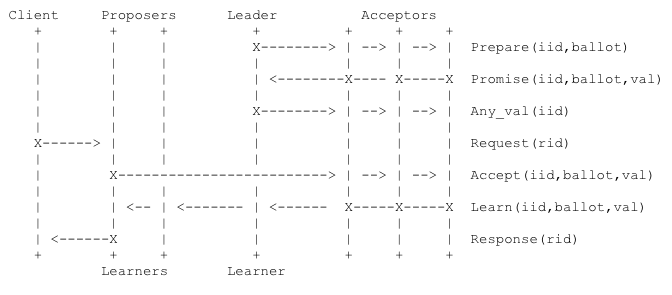
\includegraphics[width=160mm]{FP_no-conflict.png}
\caption{Normal operation of Fast Paxos Protocol}
\label{normalpax}
\end{figure}

\subsubsection{Phase 1a}
As shown in \textbf{Figure \ref{normalpax}}, Leader on start up and on regular timeouts, sends a phase 1a batch message $PREPARE<ballot, iids>$ to acceptors for $N$ (configurable) $iids(instance\_id)$. Ballot number used in this message is bigger than any ballot number used by other proposers.On receiving this batch message, acceptors do the following:
\begin{enumerate}
\item if record is not found in the acceptor log, it needs to be created with the received ballot number. 
\item if record exists, it updates the ballot number in the record found in the log to the larger ballot number (received or already present in the record).
\end{enumerate}
\noindent
After processing this message, it sends back the $PROMISE<iid, \, ballot, \, value>$ to the leader, where value could be either $NULL$ or some accepted value for that $iid$.\\

\subsubsection{Phase 1b}
\noindent 
Leader on receiving phase 1b batch message $PROMISE<iid, \, ballot, \, value>$ from acceptors do the following:
\begin{enumerate}
\item it checks for the quorum condition for given iid, if true it broadcasts the $ANY\_VAL<iid>$ batch message. This pre-executes the $Phase1$ of Classic Paxos and sets stage for Fast Paxos.
\item if the quorum condition is not reached, on timeout it resends the $PREPARE$ batch message.
\end{enumerate}

\subsubsection{Phase 2a}
\noindent
Acceptors on receiving $ANY\_VAL<iid>$ message do the following:
\begin{enumerate}
\item they update their persistent logs and set any\_enabled for each received $iid$ to true, which signifies that they can accept values from proposers directly (fast round).
\item they wait for proposers to propose values.
\end{enumerate}

\noindent
Proposers on receiving request from client, do the following:
\begin{enumerate}
\item they assign their ballot number($fixed ballot$) and send an $ACCEPT<iid, \, ballot, \, value>$ message to all acceptors directly(fast round).
\end{enumerate}

\subsubsection{Phase 2b}
\noindent
On receiving accept message, acceptors do the following:
\begin{enumerate}
\item case 1: if any enabled, they accept the message by updating their log.
\item case 2: if any is not enabled and the accept is sent by leader, they accept the value if the ballot number is greater than the one in the record.
\item in all other cases, the message is ignored (could be due to conflicts, retransmission or delayed message).
\end{enumerate}

After updating the log, acceptors broadcast the $LEARN<iid, \, value, \, ballot>$. \\
\noindent
Learners (including leader and proposers) on receiving the $LEARN$ message, do the following:
\begin{enumerate}
\item they update their in-memory log to check for duplicates and quorum condition.
\item On satisfying the quorum condition, they execute the request in the order of $iid$, deliver it (update the proposer state) and send back the response to client.
\end{enumerate}

\begin{figure}[ht!]
\centering
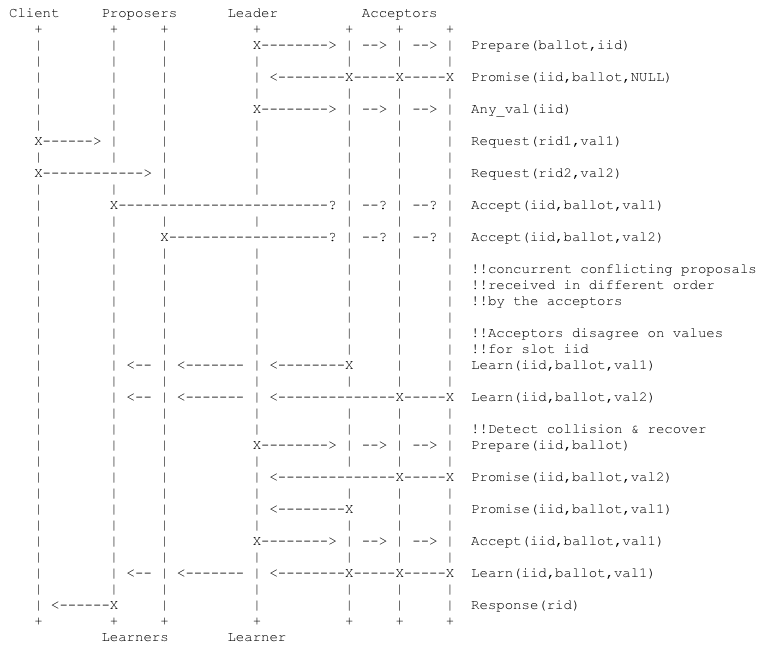
\includegraphics[width=160mm]{FP_with-conflict.png}
\caption{Conflict Resolution of Fast Paxos Protocol}
\label{conflictpax}
\end{figure}

\subsection{Resolving conflicts:}

As shown in \textbf{Figure \ref{conflictpax}}, conflicts may happen if all of the following events happen:

\begin{enumerate}
\item All acceptors received $ANY\_VAL$ message for a given $iid$
\item More than two proposer send $ACCEPT$ message with different value for that $iid$
\item None of those $LEARN$ messages reach the quorum condition, which depends on the arrival order of $ACCEPT$ messages on acceptor side (acceptor only accepts the value in the first $ACCEPT$ message received). 
\end{enumerate}

\noindent
The leader detects the progress of the protocol periodically using a timeout mechanism, if nothing gets delivered from learner, 
\begin{enumerate}
\item It broadcasts a $PREPARE<ballot,\,currrent\_iid>$, where current\_iid is the next iid to deliver by learner, and $ballot$ is a higher ballot number to indicate its conflict resolution purpose. 
\item Acceptors upon receiving $PREPARE<ballot,\, currrent\_iid>$, reply with $PROMISE<iid,\, value\_ballot,\, accepted\_value>$.
\item The leader upon receiving the $PROMISE<iid,\, value\_ballot,\,\\ accepted\_value>$, updates its in-memory records and check the quorum condition, if true, it picks the value with the highest $value\_ballot$ and broadcasts the $ACCEPT<iid, \, ballot,\, chosen\_value>$ to acceptors
\item Acceptors upon receiving this $ACCEPT<iid, \, ballot,\, chosen\_value>$ message, the condition of case 2 in $2.3.4$ will be true and the value is accepted and learn message will be broadcasted as normal. 
\item Eventually one of the proposers will get notified by learners that its proposal is granted, other proposers (losers) will retry with next $iid$ by broadcasting $ACCEPT<iid+1, \, ballot, \, value>$ nessage to acceptors
\end{enumerate}

\subsection{Retransmissions:}
There are several retransmissions in the protocol to ensure liveness and tolerate message losses:
\subsubsection{Leader $PREPARE$ retransmission:}
Leader maintains a state of all the expected $PROMISE$ messages for all $PREPARE$ messages. On timeout, leader rebroadcasts the $PREPARE$ messages for those $PROMISE$ messages for which the quorum condition is not satisfied.
\subsubsection{Learners $LSYNC$ message:}
Learner maintains a state of all the expected $LEARN$ messages, and sends $LSYNC$ message for all $iids$ for which quorum condition is not satisfied. \\

\noindent Acceptor on receiving this message will reply with $LEARN<iid,\, \\accepted\_value,\, ballot>$ for each iid.

\subsubsection{Proposers $ACCEPT$ retransmission:}
Proposer maintains the state of the current value it is trying to propose and retransmit it on timeout. The timeout will be cancelled if the value get delivered.

\subsubsection{Client request retransmission:}
Each proposer can only handle one client at a time, so if a proposer receives requests from another client while it is processing a client's request, it simply drops the message. Client on timeout, retransmits the request.

\section{Implementation Differences:}

\begin{enumerate}
\item  In \textit{Libfastpaxos}, each role is a separate process. Each proposer spawns a learner thread and main thread acts as proposer. One of the proposers (pre-defined) acts as a leader and each acceptor is a process of its own. In our implementation, there's only one entity called \texttt{paxserver} that acts as leader, learner, acceptor and proposer.
\item They use real time to do timeouts using \texttt{libevent} library whereas simulator has a different notion of time and we use counters in each instance to do timeouts.
\item They use Berkley DB as a persistent log in acceoptors whereas we use in-memory \texttt{paxlog} as our acceptor log.
\item In \textit{Libfastpaxos}, client and proposer are running as two threads in same process and using shared variables for synchronization. Hence, they cannot have multiple clients connecting to same proposer, and each proposer has a predefined FIFO request queue. In our implementation, client is independent of the paxos server system and communicates using message passing. Request may duplicate over different proposers. In proposer deliver call back, we use request id and client id instead of proposer id to detect if proposer needs to repropose its request with a higher instance id.
\end{enumerate}

\section{Test and Results:}
\begin{figure}[ht!]
\centering
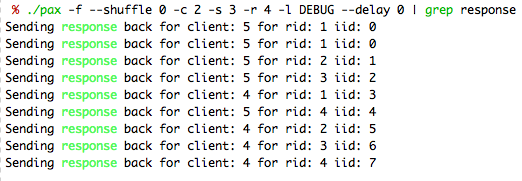
\includegraphics[width=160mm]{base_case.png}
\caption{Client's view for base case}
\label{basecase1}
\end{figure}


\begin{figure}[ht!]
\centering
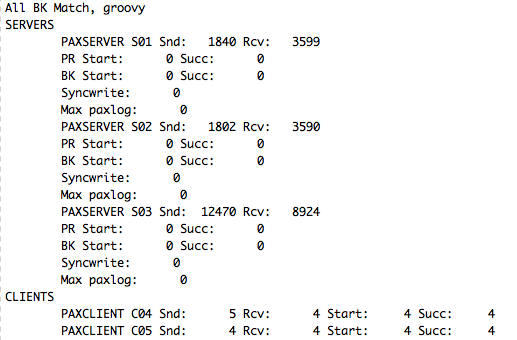
\includegraphics[width=160mm]{base_case2.png}
\caption{Paxos internal execution statistics}
\label{basecase2}
\end{figure}


\subsection{Base Case: \texttt{2 clients, 3 servers, no delay or shuffle, requests 4} }
This is the bare minimum configuration since there are no delays or shuffle, there will be no conflicts (conflict condition 3 of 2.4 will not be true). 

Figure \ref{basecase1}, shows the response being sent to clients from servers (proposers). It shows that all 6 requests from different clients are executed in a fixed global order. Figure \ref{basecase2} shows that the logs are same on all 3 servers (acceptors).

\begin{figure}[ht!]
\centering
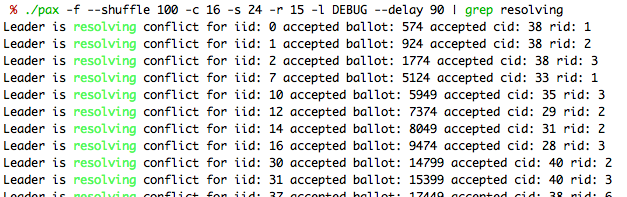
\includegraphics[width=160mm]{conflicts.png}
\caption{Part of the log showing conflicts being resolved by Leader}
\label{conflicts}
\end{figure}


\subsection{Extreme Case: \texttt{16 clients, 24 servers, 100 shuffle, 90 delay } }
Due to high shuffle and number of clients, there are higher number of conflicts and Figure \ref{conflicts} shows the conflicts being resolved by the leader.

\begin{figure}[ht!]
\centering
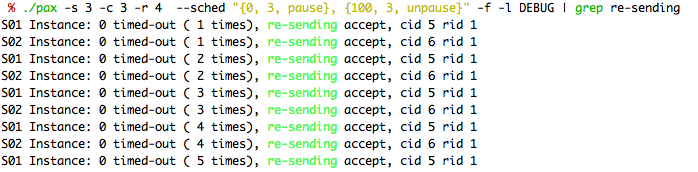
\includegraphics[width=160mm]{resending.png}
\caption{Part of the log showing conflicts being resolved by Leader}
\label{resending}
\end{figure}

\subsection{leader paused and unpaused:}
Figure \ref{resending} shows the case where leader is paused and then unpaused. During the time leader is paused, all live servers (proposers) keep retrying the accept message and as soon as leader comes back online, the protocol makes progress.

\section{Timeouts}
\subsection {Different types of timeout}
The progress of the protocol depends on the several timeouts being used by the protocol. There are four timeouts being used:
\begin{enumerate}
\item \textbf{Leader Phase 1 timeout:} Leader uses this timeout to send the phase 1a ($PREPARE$) batch messages to pre-execute the phase 1 of classic paxos and guarantee the progress of phase 1 in case of message loss.
\item \textbf{Leader Phase 2 timeout:} Leader uses this timeout to detect the progress of phase 2. If no progress has been made, it assumes that the conflicts happened for the current iid and it initiates the resolving conflict algorithm (section 2.4).
\item \textbf{Proposer Timeout:} Proposer uses this timeout to retransmit the $ACCEPT$ message if it doesn't see a progress for current iid (i.e., if no value has been accepted for the current iid).
\item \textbf{Learner Timeout:} Learner uses this timeout to sync its state with acceptors to learn the accepted values for iids that it might have missed.
\end{enumerate}

\subsection {Caveats:}
According to the original implementation of \texttt{libfastpaxos} for the protocol to make progress,
\begin{enumerate}
\item the message delays should not be of the same order for phase1 and phase2 timeouts.(delay $<<$ timeout interval)
\item when running in simulator, the number of messages that can be processed by each server on each tick should be proportional to the total number of messages per instance which is $O(N^2)$, where $N$ is the number of paxos servers.
\end{enumerate}

\section{Limitations and Corner Cases:}
\begin{enumerate}
\item Our paxos server system implementation does not count client as a learner, so client has no information about the granted $iids$ and next iid to try. That's the reason for client proposing value through proposers and not directly to acceptors.

\item If a client times out and tries a different proposer but the previous request of client succeeds and the new proposer fails to receive the update for that request, it will re-propose the value with new $iid$. One possible solution for this is for proposer to sync with acceptors to learn about the different requests for this client. Since we maintain a finite size log, we couldn't implement this in given time.
\end{enumerate}

\section {Future Work:}
\begin{enumerate}
\item \textbf{Smart Learners:} \texttt{Libfastpaxos} is using the fixed timeout intervals to detect the conflicts which is not optimal and can be optimized by making learners report conflicts to the leader as soon as they detect the conflict condition (multiple values being learned for same iid and quorum is not possible for any of the values).
\item Currently when a clients connects to a proposer that is already working on another request, the proposer drop the client's request without responding anything. Client eventually timeout and retries a random proposer. This could be optimized by buffering the client requests at the proposer or sending back a fail message so that client can continue with another proposer without waiting for the timeout.
\end{enumerate}

\begin{thebibliography}{100} 
\bibitem{lamport} Lamport, Leslie (May 1998). "The Part-Time Parliament" \emph{ ACM Transactions on Computer Systems 16 (2): 133–169}
\bibitem{libfastpaxos} Marco Primi and Daniele Sciascia. "libfastpaxos" \emph{\url{http://libpaxos.sourceforge.net/paxos_projects.php\#libfastpaxos}}
\bibitem{fastpaxos} Lamport, Leslie (July 2005). "Fast Paxos" \emph{}
\bibitem{flpresult} Fischer, Michael J; Nancy A. Lynch; Michael S. Paterson (April 1985)  "Impossibility of distributed consensus with one faulty process". \emph{Journal of the ACM 32}
\end{thebibliography} 

\end{document}